%%%%%%%%%%%%%%%%%%%%%%%%%%%%%%%%%%%%%%%%%%%%%%%%%%%%%%%%%%%
% --------------------------------------------------------
% Rho
% LaTeX Template
% Version 2.1.1 (01/09/2024)
%
% Authors: 
% Guillermo Jimenez (memo.notess1@gmail.com)
% Eduardo Gracidas (eduardo.gracidas29@gmail.com)
% 
% License:
% Creative Commons CC BY 4.0
% --------------------------------------------------------
%%%%%%%%%%%%%%%%%%%%%%%%%%%%%%%%%%%%%%%%%%%%%%%%%%%%%%%%%%%

\documentclass[9pt,a4paper,twoside]{rho-class/rho}
\usepackage[english]{babel}

%% Spanish babel recomendation
% \usepackage[spanish,es-nodecimaldot,es-noindentfirst]{babel}

\setbool{rho-abstract}{true} % Set false to hide the abstract
\setbool{corres-info}{true} % Set false to hide the corresponding author section

%----------------------------------------------------------
% TITLE
%----------------------------------------------------------

\journalname{Molecular Ecology}
\title{Genomic Evidence for Altitude-Driven Adaptive Divergence In The Color-Polymorphic Bush Cricket \textit{Isophya rizeensis}}

%----------------------------------------------------------
% AUTHORS AND AFFILIATIONS
%----------------------------------------------------------

\author[1]{Ufuk Topalan}
\author[2]{Arda Cem Kuyucu}
\author[1]{Salwa Ahmed Farid}
\author[2]{Selim Süalp Çağlar}
\author[1,$\star$]{İsmail K. Sağlam}

%----------------------------------------------------------

\affil[1]{Department of Molecular Biology and Genetics, Koç University, Istanbul, Türkiye}
\affil[2]{Department of Biology, Hacettepe University, Ankara, Türkiye}
\affil[$\star$]{corresponding author}

%----------------------------------------------------------
% DATES
%----------------------------------------------------------

\dates{This manuscript was compile on February 13, 2025}

%----------------------------------------------------------
% FOOTER INFORMATION
%----------------------------------------------------------

\leadauthor{Topalan et al. 2025}
\smalltitle{Altitude-Driven Adaptive Divergence}

%----------------------------------------------------------
% ARTICLE INFORMATION
%----------------------------------------------------------

\corres{İsmail K. Sağlam}
\email{iksaglam@ku.edu.tr}

%----------------------------------------------------------
% ABSTRACT
%----------------------------------------------------------

\begin{abstract}
    Understanding how environmental gradients shape genetic variation is fundamental to evolutionary ecology. \textit{Isophya rizeensis}, an endemic bush cricket distributed along the Fırtına Valley of Türkiye, exhibits striking altitudinal color polymorphism, making it an ideal system for studying local adaptation. Using genome-wide RAD-seq data from 71 individuals across and altitudinal gradient ($450–2300$ m elevation), we identified $92,048$ polymorphic loci, including $1,113$ putatively adaptive SNPs. Despite low genome-wide differentiation ($F_{ST} < 0.05$), adaptive loci exhibited greater divergence, suggesting selection-driven genetic structuring. Genome-wide association analyses identified $101$ SNPs significantly correlated with altitude, with bidirectional allele frequency shifts indicating disruptive selection. Discriminant analysis further revealed three major-effect loci differentiating color morphs, which were also significantly associated with elevation. Our findings illustrate the interplay between selection, gene flow, and local adaptation, highlighting how environmental heterogeneity structures genomic variation in montane ecosystems. These results provide insights into the genetic basis of phenotypic divergence and contribute to understanding biodiversity persistence under changing environmental conditions.
\end{abstract}

%----------------------------------------------------------

\keywords{Disruptive selection, Genetic Discrimination, Genotype-Environment Association, RAD sequencing}

%----------------------------------------------------------

\begin{document}
	
    \maketitle
    \thispagestyle{firststyle}
    % \tableofcontents
    \linenumbers

%----------------------------------------------------------

\section{Introduction}

    Environmental gradients, such as altitudinal and latitudinal shifts, serve as powerful natural laboratories for studying the processes shaping genetic and phenotypic variation in populations (\cite{Wogan2018}; \cite{Kelly2019}). These gradients provide key insights into the interplay between environmental factors and genetic diversity, shedding light on the forces driving local adaptation (\cite{Muir2014}). By examining phenotypic and genetic variation along these gradients, researchers can identify traits and genetic loci associated with survival in varying environments, offering a deeper understanding of the evolutionary and adaptive basis of biodiversity (\cite{Merilä2014}; \cite{Waldvogel2020}).
    
    Altitudinal gradients are particularly valuable for exploring these dynamics due to their steep environmental transitions over short geographic distances (\cite{Chown2003}; \cite{Flatt2016}). These gradients impose diverse selective pressures, including temperature, humidity, and resource availability, which can shape genetic differentiation through mechanisms such as isolation by distance (IBD) and local adaptation (\cite{Sexton2014}; \cite{Stankowski2017}; \cite{Bradburd2019}). Notably, studies combining altitudinal clines with genotype-environment association analyses have identified genetic regions linked to climatic parameters, further advancing our understanding of spatially varying selection (\cite{Hancock2011}; \cite{Slatyer2014}; \cite{Pluess2016}). Clinal variation, which manifests as gradual changes in traits or allele frequencies across environmental gradients, is an effective lens for examining the genetic underpinnings of local adaptation and response of organisms to environmental change (\cite{Mayekar2022}; \cite{Tyrmi2020}; \cite{Soliani2020}).
    
    One particularly well-documented form of clinal variation is adaptive color polymorphism in invertebrates, which often correlates with temperature and habitat variation. Color in insects, for example, can influence thermoregulation, camouflage, and ecological niche partitioning, conferring advantages such as broader resource use, greater stability, and resilience to environmental changes (\cite{Forsman2008}; \cite{Zeuss2014}; \cite{Kozlov2022}). Thermal melanism, where darker individuals warm faster in cold environments, is a well-known example of how environmental conditions, particularly temperature, can shape phenotypic variation (\cite{Clusella-Trullas2020}). While this pattern is widely observed, deviations in many ectotherms suggest that additional ecological factors, such as predation pressure or habitat complexity, may also play a role (\cite{Karlsson2008}; \cite{Goodman2021}).
    
    Beyond thermoregulation, adaptive color polymorphism enables populations with alternative color morphs to occupy distinct ecological niches, facilitating expanded distribution capacity and higher resilience to local extinctions compared to less variable species (\cite{Forsman2008}; \cite{Wennersten2009}; \cite{Kozlov2022}). This highlights the evolutionary significance of geographic variation in coloration and the importance of understanding its genetic basis. Such insights not only guide conservation strategies by identifying populations at risk (\cite{Forsman2016}) but also deepen our understanding of how evolutionary and ecological processes drive population differentiation and speciation (\cite{McLean2014}).
    
    The bush cricket \textit{Isophya rizeensis} (\cite{SEVGILI2003}), endemic to the Pontic Mountains of Turkey (Figure $1$), represents a model organism for studying these processes. This species inhabits a sharp altitudinal gradient ($300$–$2,200$ meters) and exhibits striking dorsal color polymorphism in males, with darker individuals (found at lower altitudes) transitioning to paler morphs at higher elevations (\cite{Çağlar2014}) (Figure $1$). Interestingly, this pattern contradicts the thermal melanism hypothesis, which associates dark coloration with higher, cooler habitats (\cite{CLUSELLATRULLAS2007}). Ecological and physiological studies in \textit{I. rizeensis} suggest that darker morphs warm faster and reach higher body temperatures than their pale green counterparts, which may be disadvantageous in subalpine habitats where surface temperatures can exceed 40°C due to intense solar radiation (\cite{Kuyucu2016}). In these environments, paler coloration could be an adaptation to avoid overheating, offering a survival advantage in sparsely vegetated, thermally variable conditions. Despite these observations, the genetic basis of color polymorphism and its relationship with altitude remains poorly understood. Moreover, whether this phenotypic divergence is accompanied by population-level genetic differentiation driven by selection or neutral processes is an open question.
    
    In this study, using genome-wide sequencing data with high-resolution population genetic analyses we test the hypothesis that altitude-driven selection maintains color polymorphism in \textit{I. rizeensis}. Specifically, we aimed to: 
  
    \begin{enumerate}
    \item Characterize population structure and connectivity along an altitudinal gradient.
    \item Quantify neutral vs. adaptive genetic differentiation to disentangle drift from selection.
    \item Identify loci associated with altitude and color polymorphism, clarifying whether these patterns arise from a common genetic background.
    \end{enumerate}

    By integrating environmental gradients, genomic variation, and phenotypic traits, our study provides insights into how selection maintains intraspecific diversity across heterogeneous landscapes. Specifically, we highlight the role of both neutral and adaptive genetic variation in shaping survival along altitudinal gradients, offering a clearer understanding of how these dynamics influence population persistence in changing environments.

\section{Materials and Methods}

    \subsection{Sample Collection and Sequencing}

       \textit{I. rizeensis} (Orthoptera: Tettigoniidae: Phaneropterinae: Barbitistini) is a univoltine color polymorphic bush cricket species endemic to the Fırtına Valley and its surroundings regions within the Pontic Mountains of the Eastern Black Sea, Türkiye (Figure $1$). Specimens for this study were collected between June and August 2006 from 11 locations along an altitudinal gradient ranging from $450$ to $2,300$ meters above sea level in the Fırtına Valley (Figure $1$) and categorized according to color as described in \cite{Çağlar2014}. DNA was extracted from the hind femura of individuals using \textsc{e.z.n.a.}® Insect DNA Kit (Omega Bio-Tek) according to the manufacturer’s protocol. Paired-end RAD libraries were constructed using the PstI restriction enzyme, following the protocol detailed in \cite{Ali2016}. Sequencing was conducted at an average depth of 10X on an Illumina HiSeq4000 at the UC Davis Genome Center core facilities. In total we generated RAD sequencing data from $75$ \textit{I. rizeensis} individuals along the Fırtına Valley, averaging $5-7$ individuals per location/altitude.
    
    \subsection{Alignment and filtering}

        Due to the absence of a reference genome for \textit{I. rizeensis} or in a closely related species, we generated a de novo RAD sequence reference library following the custom procedure given in \cite{SağlamMolEcol2016} (for details see supplementary materials). Raw reads from each individual were aligned to the this set of reference RAD-contigs using the \textsc{bwa-mem} algorithm (\cite{Li2010}; \cite{Li2013}). Resulting \textsc{sam} files were converted to coordinate-sorted \textsc{bam} files using \textsc{samtools} (\cite{Danecek2021}), and duplicate reads were marked with \textsc{Picard tools} (http://broadinstitute.github.io/picard). Paralog regions were identified using the \textsc{ngsParalog} (https://github.com/tplinderoth/ngsParalog) and removed from subsequent analysis.

    \subsection{SNP discovery and genotyping}

        Polymorphic sites were identified using \textsc{angsd}  (\cite{Korneliussen2014}) by calculating genotype likelihoods (\texttt{-GL $1$}), major and minor alleles (\texttt{-doMajorMinor $1$}), minor allele frequencies (\texttt{-doMaf $1$}), and generating \textsc{BCF/VCF} files (\texttt{-doBcf $1$}). Polymorphic sites were filtered to include only those with a minor allele frequency (MAF) of $0.05$ or higher (\texttt{-minMaf 0.05}). Additional filtering parameters included a minimum base quality score of $20$ (\texttt{-minQ $20$}), a minimum mapping quality of $10$ (\texttt{-minMapQ $10$}), and a posterior genotype probability threshold of $0.85$ (\texttt{-postCutoff $0.85$}). Only properly paired reads ( \texttt{-only\_proper\_pairs $1$}) were considered, and sites were retained only if the probability of them being polymorphic was statistically significant (\textit{P} < $10^{-12}$). Finally we filtered out any site that had an average per individual read depth under $6X$ and was not present in at least $50\%$ of individuals in each population.

    \subsection{Population Genetic Structure}

        Population genetic structure was assessed using Principal Component Analysis (PCA). First, a genetic covariance matrix was calculated between individuals in \textsc{PCAngsd} (\cite{Meisner2018}) based on genotype likelihoods. The covariance matrix was then subjected to eigenvalue decomposition in R (\cite{R2024}, version 4.2.0) to extract the principal component axes summarizing genetic variation and the first two principal components (PCs) were visualized in R.
       
        Admixture analyses were conducted with \textsc{NgsAdmix} (\cite{Skotte2013}) to estimate individual ancestry proportions based on genotype likelihoods. Analyses were performed for K values ranging from $2-5$, with $10$ independent runs for each K value to account for stochastic variation and avoid convergence to local optima. The most likely number of clusters was identified using the $\Delta{K}$ method of \cite{Evanno2005}, which calculates the rate of change in log-likelihood values across successive K values and admixture proportions for each K value were visualized in R.

    \subsection{Genetic Differentiation and Isolation By Distance (IBD)}

        Genetic differentiation was assessed by calculating pairwise $F_{ST}$ values between populations. Genome-wide $F_{ST}$ estimates were derived using \textsc{Angsd}, beginning with the calculation of the joint site frequency spectrum (2D-SFS) for each population pair. Global weighted $F_{ST}$ values were then computed with the \texttt{realSFS} module (\cite{Nielsen2012}). To evaluate patterns of isolation by distance (IBD), a Mantel test was performed to assess the correlation between geographic and genetic distances. A Euclidean distance matrix between populations was generated using the \textsc{Geographic Distance Matrix Generator} v1.2.3 (\Cite{Ersts2024}) and served as the predictor variable, while the linearized pairwise $F_{ST}$ matrix [$F_{ST}$/(1 - $F_{ST}$)] was used as the response variable. IBD patterns were analyzed through Pearson and Spearman correlation Mantel tests with 999 permutations, implemented in R using the \texttt{vegan package} (\cite{Oksanen2001}; \cite{Mantel1967}).
 
    \subsection{Comparing Neutral and Adaptive Genetic Variation}

        To identify putatively adaptive loci, we used the \texttt{pcadapt} function in \texttt{PCAngsd} (\cite{Meisner2018}), which detects outliers based on population structure (\cite{Luu2017}). The analysis was conducted using the Mahalanobis distance statistic across principal components, with significance determined by a chi-square ($\chi^2$) distribution with $K$ degrees of freedom based on the number of significant PC axes after correcting for multiple testing. We identified one significant principal component ($K = 1$) based on Velicier’s minimum average partial (MAP) test (\cite{Shriner2011}). To mitigate inbreeding effects, SNPs deviating from Hardy-Weinberg equilibrium due to inbreeding were filtered using the \texttt{--inbreedSites} and \texttt{--inbreed} options in \texttt{PCAngsd}, yielding a final dataset of $82,976$ SNPs, resulting in a genome-wide significance threshold of $6.03 \times 10^{-7}$ ($\chi^2 = 24.903$, $df = 1$, $\alpha = 0.05$) for determining putatively adaptive loci.

        Genetic diversity was estimated separately for neutral and adaptive loci by computing pairwise nucleotide differences ($\theta_{\pi}$) based on the folded site frequency spectrum (SFS) since we did not have a suitable outgroup for determining ancestral states. Allele frequency likelihoods were first calculated in \texttt{ANGSD} (\texttt{-doSaf 1}), followed by maximum likelihood estimation of the SFS using \texttt{realSFS}. Genome-wide $\theta_{\pi}$ was obtained using the \texttt{thetaStat} module (\texttt{-do\_stat}) by averaging per-site values across all RAD loci.

        To assess genetic differentiation, pairwise $F_{ST}$ values were calculated, and isolation by distance was evaluated via Mantel tests, correlating geographic and genetic distances separately for neutral and adaptive loci.


    \subsection{Genetic Variation Associated with Altitude}
    
        To investigate genetic variation associated with altitude, a genome-wide association study (GWAS) was conducted using score statistics (\texttt{-doAsso $2$}) in \textsc{Angsd}. The score test applies a generalized linear model framework, with posterior genotype probabilities as the dependent variable and altitude (\texttt{-yQuant}) as the predictor variable, calculating likelihood scores for each SNP independently (\cite{Skotte2012}).

        Association mapping included the identification of polymorphic sites (\texttt{-SNP\_pval 1e-06}), inference of major and minor alleles (\texttt{-doMajorMinor $1$}), and estimation of allele frequencies (\texttt{-doMaf $1$}). Stringent filtering criteria were applied to exclude SNPs with a minor allele frequency below $5\%$ (\texttt{-minMaf $0.05$}) or fewer than ten observations per genotype class (homozygous major, heterozygous, and homozygous minor; \texttt{-minHigh $10$}). Likelihood ratio test (LRT) scores for each SNP were converted to \textit{P}-values, assuming a chi-square ($\chi^2$) distribution with one degree of freedom. A Bonferroni correction was applied to control for multiple testing.
        
        To examine allele frequency patterns at significantly associated sites, the frequency of the reference allele (defined as the minor allele across the entire dataset) was plotted against altitude. This analysis highlights altitude-driven genetic variation by illustrating changes in allele frequencies with elevation.

    \subsection{Genetic Discrimination of Color Morphs}
        To investigate genetic variation associated with color morphs, a Discriminant Analysis of Principal Components (DAPC) was performed using the R package \texttt{adegenet} (v2.1.1; \cite{Jombart2008}; \cite{Jombart2011}). Genotypes were called in \textsc{Angsd} (\texttt{-doGeno $4$}) and exported as \texttt{VCF/BCF} files (\texttt{-doBcf $1$}) using a uniform prior (\texttt{-doPost 2}) and a posterior probability cutoff of $85\%$ (\texttt{-postCutoff $0.85$}). The DAPC retained principal component axes explaining up to $80\%$ of the variance, with color morph (dark vs. pale) specified as the grouping variable.
        
        To identify SNPs contributing most strongly to discrimination between color morphs, variable contributions of SNPs to the linear discriminant functions were examined. These contributions were hierarchically clustered using the \texttt{Average} method in the \texttt{snpzip} function of \texttt{adegenet}, grouping loci into "outlier" and "non-outlier" categories.
        
        Genotypic variation at the identified outlier loci was further explored by categorizing individuals based on genotypes either as heterozygous, homozygous for the minor allele, or homozygous for the major allele. Genotype distributions were visualized as a heatmap generated with \texttt{ggplot2} (\cite{ggplot2}), illustrating differences in genotypic states between dark and pale morphs.

\section{Results}

    \subsection{Alignment statistics and SNP discovery}

        Using our de novo reference assembly strategy, we identified $224,187$ unique RAD-loci ranging from $250$ to $800$ bp, with an average length of $324$ bp. Raw read alignments to the de novo set of reference RAD-contigs achieved a mapping success rate of $73\%$ to $83\%$, averaging $77\%$, with a mean individual read depth of approximately $5-6X$. Detailed data on raw read counts, raw alignments, and alignments after removing PCR duplicates are provided in Supplementary Table S1. Based on alignment statistics, we excluded individuals with fewer than $1,000,000$ aligned reads after all filters, resulting in a final dataset of $71$ individuals from $11$ locations (Table 1). Across all collection sites, we identified $9,616$ polymorphic loci and $92,048$ high-confidence SNPs (\textit{P} < $10^{-12}$) with a minor allele frequency $>0.05$, a minimum per individual read dept of $6X$ and present in $\geq50\%$ of individuals per population.
        
\begin{table}[!h]
    \small
    \captionsetup[table]{labelsep=space, 
        justification=raggedright, singlelinecheck=off}
    \caption{Altitude, coordinates, color category and samples sizes of \textit{I. rizeensis} used in this study.}
    \label{tab:my-table}
    \scalebox{1.3}{
    \begin{tabular}{@{}lllll@{}}
    \toprule
    Altitude (m) & Latitude & Longitude & Color & N \\ \midrule
    450          & 40.9856  & 40.9646   & DARK  & 7 \\
    850          & 40.9406  & 40.9850   & DARK  & 6 \\
    900          & 40.9166  & 40.9456   & DARK  & 7 \\
    1000         & 40.9075  & 40.9479   & DARK  & 7 \\
    1100         & 40.8880  & 40.9297   & PALE  & 7 \\
    1200         & 40.8630  & 40.9342   & PALE  & 5 \\
    1300         & 40.8638  & 40.9501   & PALE  & 5 \\
    1900         & 40.8548  & 41.0125   & PALE  & 7 \\
    2000         & 40.7998  & 40.9217   & PALE  & 7 \\
    2100         & 40.7995  & 40.9588   & PALE  & 7 \\
    2300         & 40.7915  & 40.9574   & PALE  & 6 \\ \bottomrule
    \end{tabular}%
    }
\end{table}

    \subsection{Population Genetic Structure and Differentiation}

        Principal Component Analysis (PCA) identified two distinct genetic clusters along PC1, corresponding to individuals from lower (dark-colored) and higher (pale-colored) altitudes (Figure 2A). However, PC1 and PC2 accounted for only $3.82\%$ and $2.08\%$ of the total genetic variation, respectively, indicating limited overall genetic divergence. A transitional zone was observed along PC1, comprising individuals from intermediate altitudes (1100–1900 meters).
        
        Admixture analysis, consistent with the PCA, identified K=3 as the optimal number of clusters (Supplementary Figure S1). Low and high altitude populations showed minimal admixture, predominantly belonging to distinct genetic ancestries whereas mid-altitude populations (1100–1900 meters) formed a transition zone with mixed ancestry, corroborating PCA findings (Figure 2B). Along the altitudinal gradient, the proportion of low-altitude ancestry (black) decreased, while high-altitude ancestry (green) increased, reflecting a reciprocal relationship between genetic components and elevation (Figure 2B).

        Pairwise $F_{ST}$ comparisons revealed relatively low genetic differentiation along the altitudinal gradient and between populations (< $0.05$), indicating substantial genetic connectivity across the landscape (Supplementary Figure $S2$). Despite the overall low divergence a Mantel test revealed a significant relationship between linearized $F_{ST}$  [$F_{ST}/(1 - F_{ST})$] values and geographic distance for both Pearson (\textit{$r_p$} = $0.838$, \textit{P} = $0.001$) and Spearman (\textit{$r_s$} = $0.869$, \textit{P} = $0.001$) correlation tests, indicating a clear pattern of IBD (Figure 2C).

    \subsection{Comparing neutral and adaptive variation}

        \textsc{PCAdapt} identified $1,113$ putatively adaptive SNPs within 809 distinct RAD-loci and $81,863$ neutral SNPs within 8699 distinct RAD-loci. Genome-wide mean genetic diversity ($\theta_\pi$) was generally high across the altitudinal gradient, ranging from $0.058$ to $0.065$ (Figure $3A$, Table $S2$). Mean genetic diversity values for neutral and adaptive loci were largely similar along the altitudinal gradient. However, we observed a slight increase in neutral genetic diversity relative to adaptive genetic diversity at mid-altitudes (excluding $1,000$ meters), with significant differences in mean $\theta_\pi$ between $900$ and $1,900$ meters (Figure 3A, Table S2).
    
        To compare genetic divergence, separate Mantel tests assessed correlations between geographic distance and linearized $F_{ST}$ [$F_{ST}$/(1 - $F_{ST}$) for adaptive and neutral loci. Genetic divergence increased with geographic distance for both categories, but the relationship was significantly steeper for adaptive loci (\textit{$r_p$} = $0.91$, \textit{$r_s$} = $0.91$, \textit{$P$} = $0.001$) compared to neutral loci (\textit{$r_p$} = $0.84$, \textit{$r_s$} = $0.87$, \textit{$P$} = $0.001$) (Figure 3B). These results indicate greater divergence and signs of allelic fixation in adaptive loci at altitudinal extremes compared to neutral loci, suggesting a stronger role for selection in driving genetic differentiation along the altitudinal gradient.

    \subsection{Association mapping of altitudinal variation}

        Genome-wide association studies using altitude as a quantitative variable was based upon $53,901$ SNPs that passed all filters leading to a genome wide significance of $9.276\times10^{-7}$ ($\alpha = 0.05$; LRT > $24.07$). Based on this threshold we identified 101 SNPs within 75 unique RAD-loci significantly associated with genetic variation along the altitudinal gradient (Table S3). Out of the 75 unique RAD-loci 73 were classified as "putatively adaptive" in prior analysis (Table S3). Notably, allele frequency changes showed a bidirectional pattern, with some loci displaying increased minor allele frequencies at low altitudes, while others increased at high elevations (Figure 4, Table S3). These opposing frequency shifts suggest that selection is acting on different genetic variants across the gradient, potentially reflecting locally adapted alleles in lowland vs. highland populations.
        
    \subsection{Genetic Discrimination between Color Morphs}

        Discriminant analysis of principal components (DAPC) based on dark and pale color morphs clearly separated individuals into two groups along the first discriminant function (DF1), with a high posterior assignment probability (0.97; Figure 5A). Pale individuals were perfectly classified (posterior success = 1.0), while $92.6\%$ of dark individuals were correctly assigned, with only two misclassified as pale.
   
        DF1 loadings identified three major-effect loci significantly contributing to genetic discrimination between color morphs (Figure 5B). These loci displayed bimodal genotype distributions, with pale individuals nearly fixed for the major allele and dark individuals predominantly heterozygous (Figure 5C). Notably, these loci were also significantly associated with altitude (Table S3), reinforcing the connection between color polymorphism and altitudinal variation.


\section{Discussion}

This study provides the first detailed analysis of the genetic basis of color polymorphism in \textit{I. rizeensis} along an altitudinal gradient. Our findings illustrate how altitude acts as a selective force, shaping genetic variation at loci associated with coloration and driving both local adaptation and genetic differentiation. More broadly, this work offers insights into the maintenance of adaptive polymorphism in response to environmental gradients, contributing to a deeper understanding of how natural selection influences genetic diversity in wild populations.

\subsection{Contrasting Patterns of Neutral and Adaptive Genetic Variation}

Despite the high connectivity across the altitudinal gradient (pairwise $F_{ST}  <0.05$), our analysis revealed distinct patterns between adaptive and neutral loci. Neutral loci exhibited relatively uniform diversity across populations, with only slight fluctuations along the gradient. Mid-altitude populations showed slightly increased neutral genetic diversity, likely due to gene flow between high- and low-altitude populations, a well-documented phenomenon in transition zones (\cite{Byars2009}; \cite{Polato2017}; \cite{Cortázar-Chinarro2017}).

In contrast, adaptive loci exhibited significantly greater differentiation along the altitudinal gradient, with the steepest divergence observed at the highest and lowest elevations. This pattern suggests that selection, rather than drift or migration, plays a dominant role in shaping differentiation at environmental extremes (\cite{Raeymaekers2017}; \cite{Cortázar-Chinarro2017}). The stronger correlation between genetic divergence and geographic distance for adaptive loci, relative to neutral markers, supports a role for isolation by environment (IBE) alongside isolation by distance (IBD). This pattern mirrors observations in other species experiencing strong environmental selection (\cite{Jiang2019}; \cite{Wagutu2022}; \cite{Wakamiya2023}) and aligns with growing evidence that environmental heterogeneity, rather than physical barriers, is the primary driver of adaptive genetic differentiation in montane species (\cite{Zancolli2019}; \cite{Wagutu2022}).

\subsection{Disruptive Selection and the Maintenance of Polymorphism}

Bidirectional allele frequency shifts at altitude-associated loci provide compelling evidence that selection maintains genetic and phenotypic variation across the gradient. The opposing allele frequency patterns at extreme elevations suggest that different loci are under selection in different environments, consistent with the action of disruptive selection (\cite{White2021}; \cite{Wadgymar2022}). Such selection may contribute to the persistence of polymorphism despite ongoing gene flow, reinforcing findings from other taxa where environmental gradients impose spatially structured selection pressures (\cite{Tigano2016}; \cite{Zancolli2019}).

Disruptive selection may be particularly important in structuring these populations by favoring different alleles at different altitudinal extremes, potentially leading to distinct adaptive peaks (\cite{Berdahl2015}, \cite{Forester2016}). In \textit{I. rizeensis}, the observed bimodal genotype distributions at key loci suggest that selection maintains alternative alleles rather than favoring an intermediate state, a pattern characteristic of polymorphisms maintained by divergent ecological selection.

\subsection{Genetic Differentiation Between Color Morphs}

Discriminant analysis (DAPC) revealed strong genetic differentiation between dark and pale morphs, with three loci significantly contributing to this separation. Pale morphs were nearly fixed for the major allele, while dark morphs were predominantly heterozygous, reflecting a bimodal genotype distribution indicative of selective pressures (\cite{Prince2017}, \cite{Thompson2019}, \cite{PereiraMartins2022}). The overlap between these loci and altitude-associated markers suggests that color polymorphism is linked to altitudinal adaptation, similar to systems where coloration is stabilized by divergent selection across microhabitats (\cite{Villoutreix2023}) or environmental gradients (\cite{Mullen2008}; \cite{Wittkopp2003}).

While the exact ecological role of coloration in \textit{I. rizeensis} remains unresolved, potential selective forces could include thermoregulation, crypsis, or pleiotropic effects linked to altitude adaptation. In \textit{Drosophila}, pigmentation is influenced by dopamine-related genes interacting with melanin synthesis pathways (\cite{Wright1987}; \cite{Wittkopp2003}), whereas in ladybirds and grasshoppers, color variation arises through distinct genetic mechanisms (\cite{MICHIE2010}; \cite{Bastide2016}). The pathways underlying color variation in \textit{I. rizeensis} likely involve complex interactions between ecological and genetic factors, requiring further investigation.

\subsection{Limitations and Future Directions}

Despite strong evidence for selection driving divergence along the altitudinal gradient, several limitations should be acknowledged. First, the absence of a reference genome for \textit{I. rizeensis} or a closely related species restricts functional inference, limiting our ability to pinpoint the exact genes underlying adaptation. Second, our inference of selection is based on spatial patterns of allele frequencies and association tests rather than rigorous genomic selection scans. The latter typically require longer sequence stretches to detect robust selection signals, which is currently not feasible in our system due to the lack of a suitable reference genome. Previous studies have highlighted the importance of genome contiguity for detecting selection signatures in non-model species (\cite{hoban2016finding}; \cite{fumagalli2013assessing}; \cite{lotterhos2019effect}), emphasizing the need for high-quality genomic resources in future work.

Future studies should prioritize functional validation through transcriptomic analyses, gene expression assays, or synteny-based comparative genomics. Additionally, experimental approaches such as reciprocal transplants or common garden experiments could directly test the fitness effects of altitude-associated alleles. Despite these gaps, our study establishes \textit{I. rizeensis} as a valuable model for investigating how environmental gradients shape adaptive genetic variation.

\section{Conclusion}

This study demonstrates that altitudinal gradients drive adaptive divergence in \textit{I. rizeensis}, likely through disruptive selection that maintains polymorphism despite gene flow. By linking allele frequency clines to both elevation and coloration, we provide a mechanistic framework for understanding biodiversity patterns in montane ecosystems. Future research integrating functional genomics and ecological assays will be crucial for identifying the molecular pathways and selective pressures driving these adaptations. Such insights will enhance our ability to predict species responses to environmental change and inform conservation strategies for montane biodiversity under shifting climatic conditions.


\section{Author Contributions}
IKS conceptualized the study with input from ACK and SSÇ. IKS, ACK, SSÇ and UT conducted field sampling. UT conducted all laboratory work and data analysis with contributions from SAF, IKS and ACK. IKS wrote the manuscript with input from UT. All authors read and approved the final version of the manuscript.

\section{Acknowledgments}
This work was supported by the The Scientific and Technological Research Council of Türkiye (TÜBİTAK), grant number 122Z038 and Hacettepe University Scientific Research Center Project No. 03 02 601 012. We are greatly thankful to Dr. Michael Ryan Miller and Dr. Sean O'Rourke for conducting RAD library preparation and sequencing at UC Davis.  

\section{Ethics Statement}
All field collections were done with approval from the General Directorate of Nature Conservation and National Parks of Türkiye under field permits E-21264211-288.04-5057102 and xxxxx.

\section{Conflicts of Interest}
Authors declare no conflict of interest.

\section{Data Availability Statement}
Raw sequence data are available from the NCBI SRA: SRRXXXXX (BioProject PRJNAXXXX). Command lines, shell and R scripts for conducting all analyses outlined in the study can be found at https://github.com/UfukTopalan/AdaptiveGenomics\_Isophya.

\printbibliography
\clearpage\section{Figures}
\begin{figure}[h]
\centering
\includegraphics[width=1.8\columnwidth]{Figure_1.pdf}
\caption{Sampling locations of \textit{I. rizeensis} in the Fırtına Valley, Türkiye. Map showing the 11 collection sites along an altitudinal gradient within the Fırtına Valley. Village names and elevation values (in meters) are indicated. Sampling locations are categorized based on the two major color morphs of \textit{I. rizeensis} dark and pale.}
\label{Figure 1}
\end{figure}

\clearpage
\newpage
\begin{figure}[h]
\centering
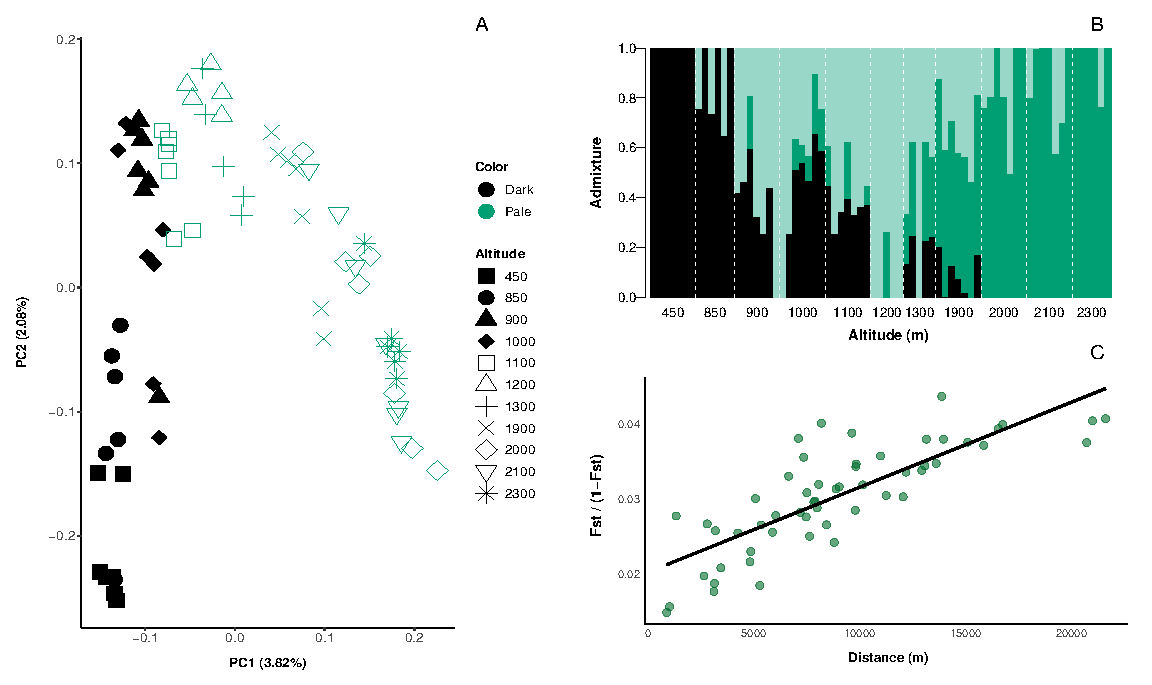
\includegraphics[width=1.8\columnwidth]{Figure_2.pdf}
\caption{Genetic structure and differentiation of \textit{I. rizeensis} along an alitudinal gradient in the Fırtına Valley. \textbf{(A)} Principal Component Analysis (PCA) of genetic variation, showing genetic structuring between lower-altitude (dark-colored) and higher-altitude (pale-colored) individuals along PC1. \textbf{(B)} Admixture proportions for $K=3$, illustrating distinct genetic ancestries at low (black) and high (green) altitudes, with mid-altitude populations exhibiting mixed ancestry. \textbf{(C)} Isolation-by-distance (IBD) pattern revealed by Mantel tests, showing significant patterns of genetic differentiation along the altitudinal gradient as measured by $F_{ST}$}
\label{Figure 2}
\end{figure}

\clearpage
\newpage
\begin{figure}[h!]
\centering
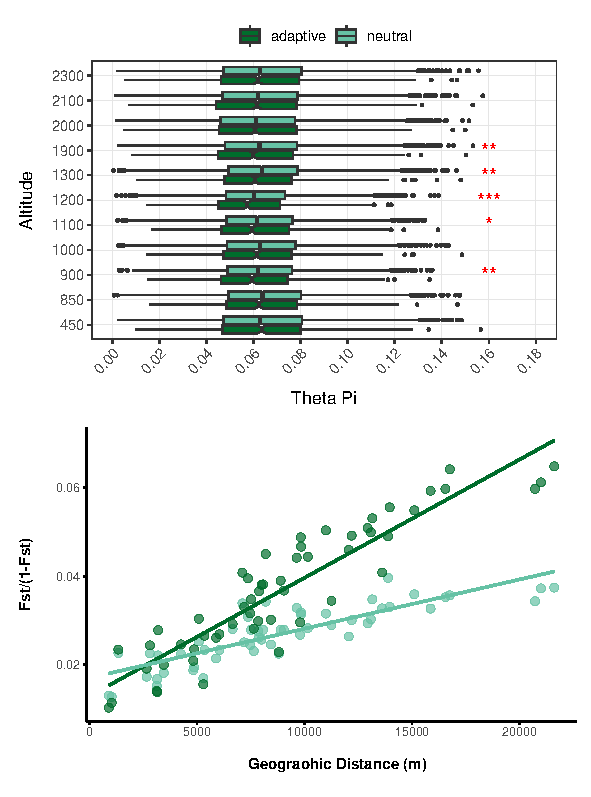
\includegraphics[width=0.8\columnwidth]{Figure_3.pdf}
\captionsetup[table]{labelsep=space, 
        justification=raggedright, singlelinecheck=off}
    \caption{Nucleotide diversity (A) and genetic differentiation (B) for adaptive and neutral loci in \textit{I. rizeensis} along an alitudinal gradient in the Fırtına Valley}
\label{Figure 3}
\end{figure}
\newpage
\begin{figure}[h!]
\centering
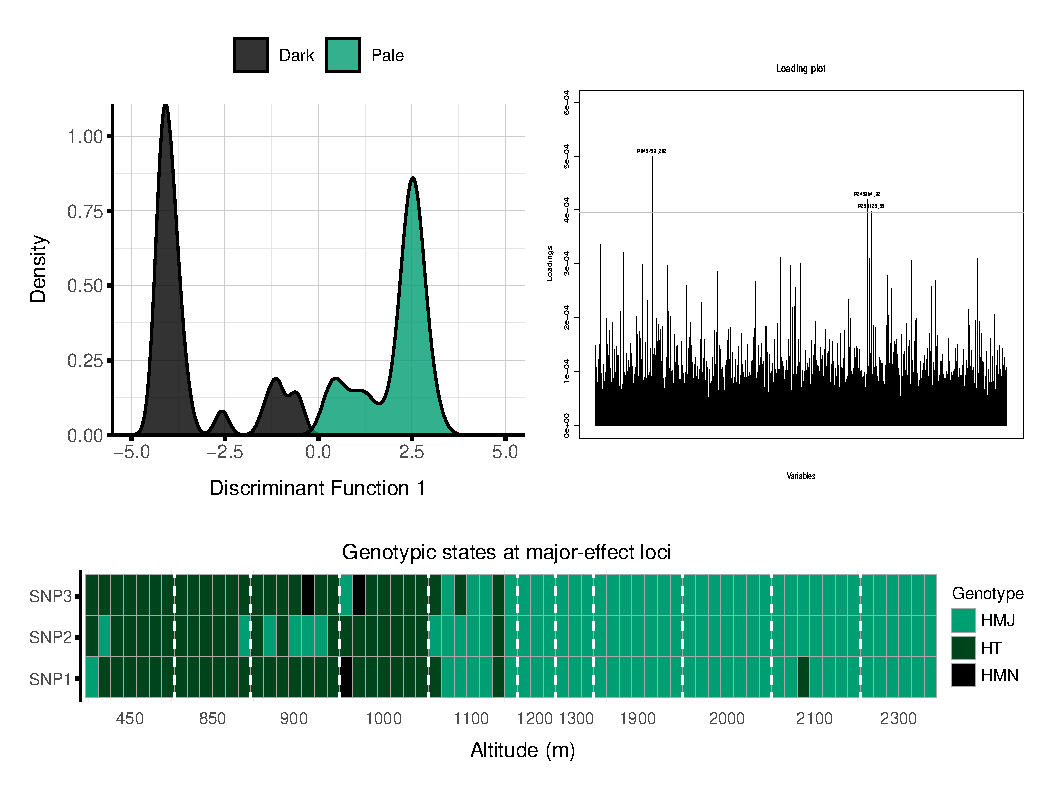
\includegraphics[width=0.8\columnwidth]{Figure_4.pdf}
\caption{Altitudinal variation in allele frequencies for the 102 SNPs significantly associated with elevation in \textit{I. rizeensis}, showing two distinct trends where the minor allele frequency either increases or decreases with altitude.}
\label{Figure 4}
\end{figure}

\begin{figure*}[b!]
\centering
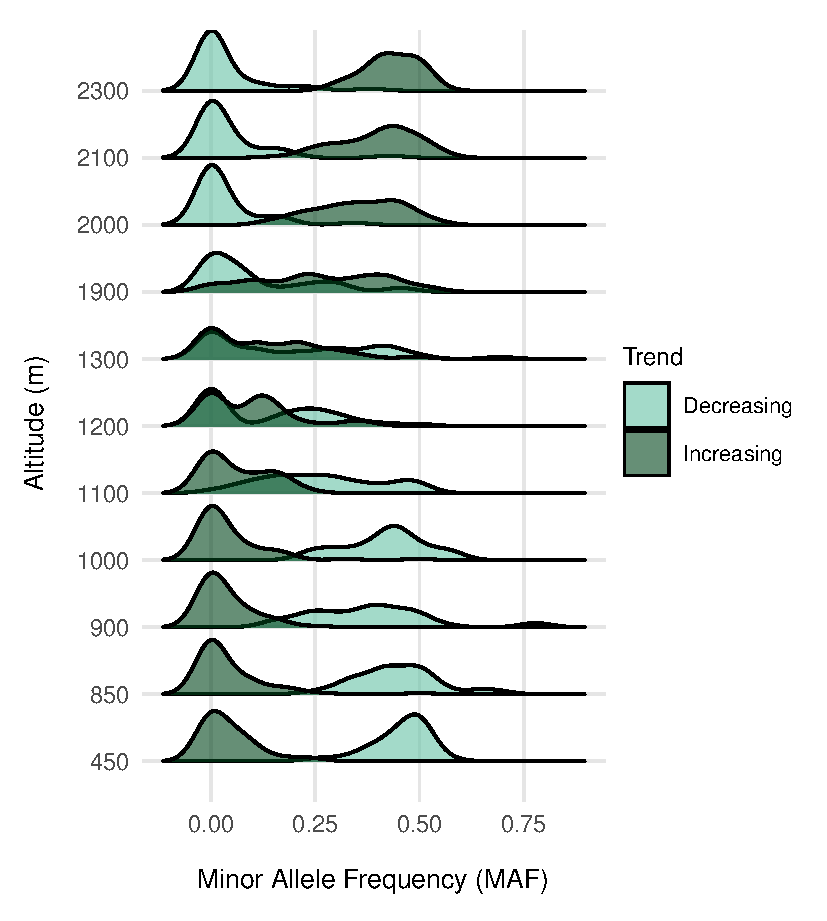
\includegraphics[width=1.8\columnwidth]{Figure_5.pdf}
\caption{Genetic differentiation between dark and pale color morphs of \textit{I. rizeensis} based on Discriminant Analysis of Principal Components (DAPC). (A) DAPC density plot along Discriminant Function 1 (DF1), showing clear separation between the morphs. (B) SNP loadings on DF1 identifying three major-effect loci contributing to morph differentiation. (C) Genotypic states at the three major loci along the altitudinal gradient.}
\label{Figure 5}
\end{figure*}

\end{document}